\documentclass{article}

%%% Fill details here (in the second brackets)
\newcommand{\name}{Xin Qiu}     % Your name (First Last)
\newcommand{\wustlkey}{qiuxin}             % Your WUSTL Key
%%%



%%%%%%%%%%%%%%%%%%%%%% Formatting Stuff %%%%%%%%%%%%%%%%%%%%%%%%%%%
\usepackage{times}
\usepackage[T1]{fontenc}

\setlength{\parskip}{1em}\setlength{\parindent}{0pt}
\linespread{1.25}
\usepackage[margin=0.7in,top=1in]{geometry}\usepackage{fancyhdr}
\pagestyle{fancy}\lhead{\bf \name}\rhead{\bf \wustlkey}\cfoot{\thepage}
\newcommand{\info}{\clearpage \subsection*{Information}}
\newcommand{\solution}[1]{\clearpage \subsection*{Solution #1}}
\newcommand{\spart}[1]{\paragraph{(#1)}}
%%%%%%%%%%%%%%%%%%%%%%%%%%%%%%%%%%%%%%%%%%%%%%%%%%%%%%%%%%%%%%%%%%%


%%% Add any more packages if you want to
\usepackage{amsmath,graphicx}


\begin{document}
%%%%% Main Body goes here

% Begin solution to every problem like this.
\solution{1} 

\spart{a}Based on the lecture 2 slide, we have:
$$
I \leftarrow gI^0 + g\sqrt{I^0}\epsilon_1 + \sqrt{(g^2\sigma^2_{2a} + \sigma^2_{2b})}\epsilon_2
$$
and we know that:
$$
I = gI^0 + \epsilon
$$
so, we have:
$$
\epsilon= g\sqrt{I^0}\epsilon_1 + \sqrt{(g^2\sigma^2_{2a} + \sigma^2_{2b})}\epsilon_2
$$
then the variance of $\epsilon$, which is $\delta^2$ is:
\begin{eqnarray*}
\delta^2 & = & (g\sqrt{I^0})^2 + (\sqrt{(g^2\sigma^2_{2a} + \sigma^2_{2b})})^2 \\
              & = & g^2I^0 + g^2\sigma^2_{2a} + \sigma^2_{2b}
\end{eqnarray*}

\spart{b}Since we know that if we chose to have a shorter exposure time $\frac{T}{k}$, the corresponding ideal intensity would also be $\frac{I^0}{k}$, and also we would scale up the amplification factor to $g \times k$, so we can have:
\begin{eqnarray*}
I & = & gk\frac{I^0}{k} + gk\sqrt{\frac{I^0}{k}}\epsilon_1 + \sqrt{({g}^2{k}^2\sigma^2_{2a} + \sigma^2_{2b})}\epsilon_2 \\
  & = & gI^0 + g\sqrt{I^0k }\epsilon_1 + \sqrt{({g}^2{k}^2\sigma^2_{2a} + \sigma^2_{2b})}\epsilon_2
\end{eqnarray*}
then the expected variance $\delta^2$ of noise $\epsilon$ is:
\begin{eqnarray*}
\delta^2 & = & (g\sqrt{I^0k })^2 + (\sqrt{({g}^2{k}^2\sigma^2_{2a} + \sigma^2_{2b})})^2 \\
              & = & g^2I^0k + g^2k^2\sigma^2_{2a} + \sigma^2_{2b}
\end{eqnarray*}

\spart{c}We know that $I = \frac{\sum^k_{i=1}I_i}{k}$, and also from (b) we know that:
$$
I_i = gI^0 + g\sqrt{I^0k }\epsilon_1 + \sqrt{({g}^2{k}^2\sigma^2_{2a} + \sigma^2_{2b})}\epsilon_2
$$
and we also know that $\delta^2_i$ is:
$$
\delta^2_i = g^2I^0k + g^2k^2\sigma^2_{2a} + \sigma^2_{2b}
$$
then, we have:
$$
\epsilon = \frac{1}{k}(\epsilon_1 + \epsilon_2 +...+\epsilon_k)
$$
so, the noise variance $\delta^2$ of this case should be:
\begin{eqnarray*}
\delta^2 & = & \frac{k}{k^2}(g^2I^0k + g^2k^2\sigma^2_{2a} + \sigma^2_{2b}) \\
              & = & g^2I^0 + g^2k\sigma^2_{2a} + \frac{1}{k}\cdot\sigma^2_{2b}
\end{eqnarray*}

\spart{d}I think it really depends. If we have a constant time budget, we need to compare two equations, which are:
$$
\delta^2 = g^2I^0 + g^2\sigma^2_{2a} + \sigma^2_{2b}
$$
and,
$$
\delta^2 = g^2I^0 + g^2k\sigma^2_{2a} + \frac{1}{k}\cdot\sigma^2_{2b}
$$
It is obviously that when $g^2k\sigma^2_{2a}$ scales up, then $\frac{1}{k}\cdot\sigma^2_{2b}$ scales down.So, in order to determine which strategy is better depends on $k$, $\sigma_{2a}$ and $\sigma_{2b}$, if $k\sigma^2_{2a} < \sigma^2_{2b}$, taking a single shot is preferable, if $k\sigma^2_{2a} > \sigma^2_{2b}$, then taking $k$ shots is preferable.

\solution{2}
The input image is shown in Figure \ref{fig:input}.
\begin{figure*}[!h]
  \centering
    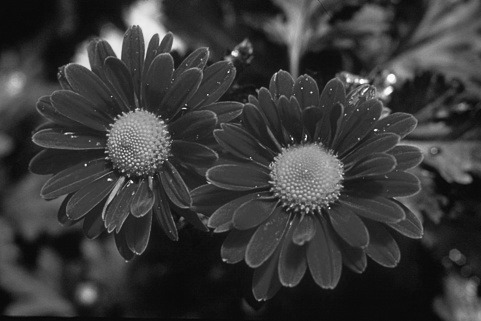
\includegraphics[height=25em]{code/inputs/p2_inp.jpg}
  \caption{Input image for problem 2.}
  \label{fig:input}
\end{figure*}
\

The output image is shown in Figure \ref{fig:output}.
\begin{figure*}[!h]
  \centering
    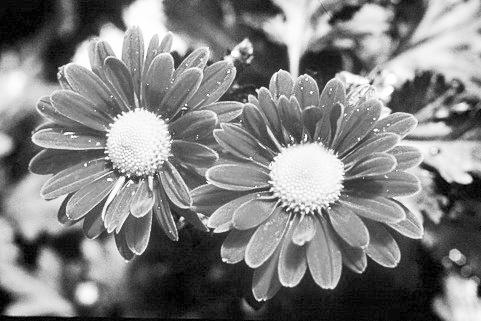
\includegraphics[height=25em]{code/outputs/prob2.jpg}
  \caption{Output image for problem 2.}
  \label{fig:output}
\end{figure*}

\solution{3}
\spart{a} The input image is shown in Figure \ref{fig:input3a} and the output image is shown in Figure \ref{fig:output3a}.
\begin{figure*}[!h]
  \centering
    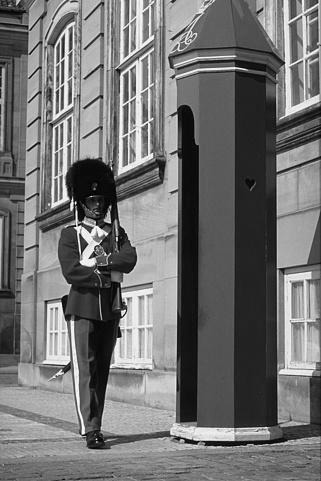
\includegraphics[height=25em]{code/inputs/p3_inp.jpg}
  \caption{Input image for problem 3a.}
  \label{fig:input3a}
\end{figure*}

\begin{figure*}[!h]
  \centering
    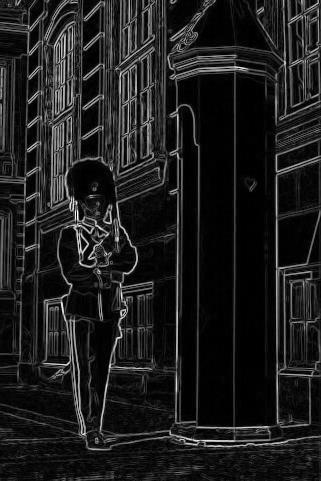
\includegraphics[height=25em]{code/outputs/prob3_a.jpg}
  \caption{Output image for problem 3a.}
  \label{fig:output3a}
\end{figure*}

\spart{b} Figure \ref{fig:output3b0} to Figure \ref{fig:output3b2} show images before NMS corresponding to three different thresholds, and Figure \ref{fig:output3bnms0} to Figure \ref{fig:output3bnms2} show image after NMS corresponding to three different thresholds.
\begin{figure*}[!h]
  \centering
    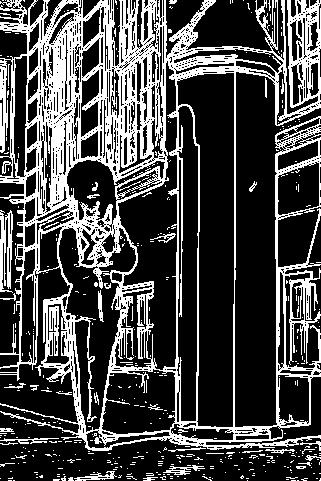
\includegraphics[height=25em]{code/outputs/prob3_b_0.jpg}
  \caption{Problem 3\_b\_0 under T0 before NMS}
  \label{fig:output3b0}
\end{figure*}

\begin{figure*}[!h]
  \centering
    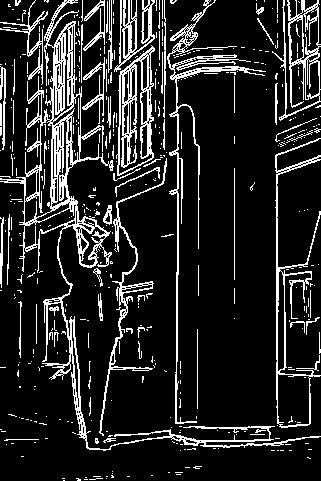
\includegraphics[height=25em]{code/outputs/prob3_b_1.jpg}
  \caption{Problem 3\_b\_1 under T1 before NMS}
  \label{fig:output3b1}
\end{figure*}

\begin{figure*}[!h]
  \centering
    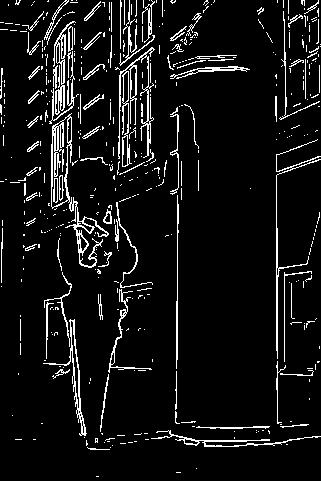
\includegraphics[height=25em]{code/outputs/prob3_b_2.jpg}
  \caption{Problem 3\_b\_2 under T2 before NMS}
  \label{fig:output3b2}
\end{figure*}

\begin{figure*}[!h]
  \centering
    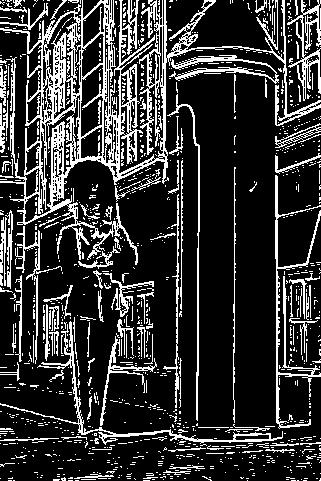
\includegraphics[height=25em]{code/outputs/prob3_b_nms0.jpg}
  \caption{Problem 3\_b\_0 under T0 after NMS}
  \label{fig:output3bnms0}
\end{figure*}

\begin{figure*}[!h]
  \centering
    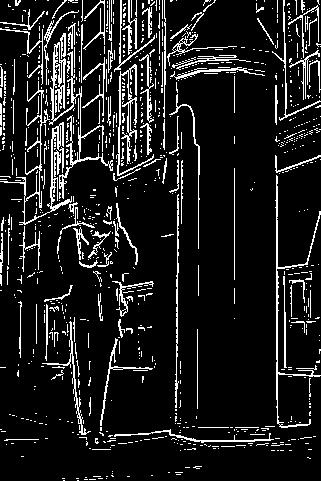
\includegraphics[height=25em]{code/outputs/prob3_b_nms1.jpg}
  \caption{Problem 3\_b\_1 under T1 after NMS}
  \label{fig:output3bnms1}
\end{figure*}

\begin{figure*}[!h]
  \centering
    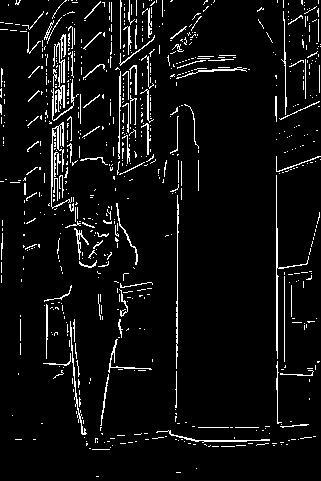
\includegraphics[height=25em]{code/outputs/prob3_b_nms2.jpg}
  \caption{Problem 3\_b\_2 under T2 after NMS}
  \label{fig:output3bnms2}
\end{figure*}

\solution{4} Figures below show the result of Bilateral filtering, Figure \ref{fig:output41a} to Figure \ref{fig:output41c}, they are affected by different parameters, and Figure \ref{fig:output41rep} shows the result of repeated bilateral filtering, smooth but blur, and Figure \ref{fig:output42rep} shows the result of more repeated time and more noise and make the image more smooth but more blur.
\begin{figure*}[!h]
  \centering
    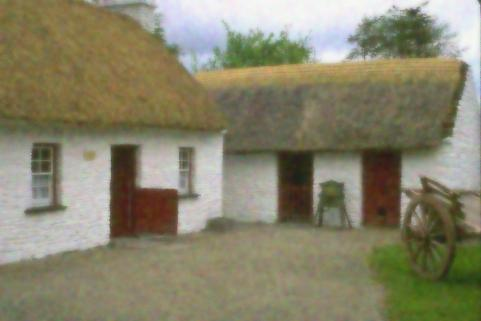
\includegraphics[height=25em]{code/outputs/prob4_1_a.jpg}
  \caption{Problem 4\_1\_a result}
  \label{fig:output41a}
\end{figure*}

\begin{figure*}[!h]
  \centering
    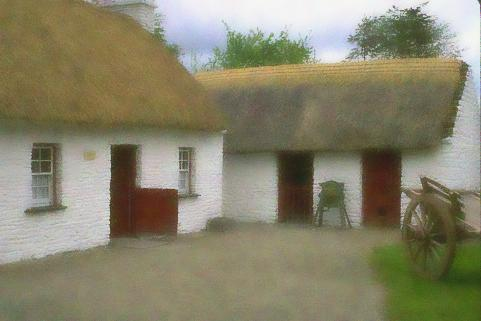
\includegraphics[height=25em]{code/outputs/prob4_1_b.jpg}
  \caption{Problem 4\_1\_b result}
  \label{fig:output41b}
\end{figure*}

\begin{figure*}[!h]
  \centering
    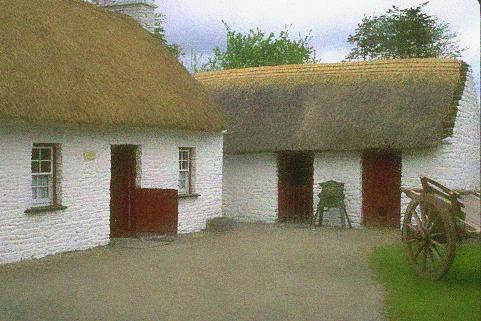
\includegraphics[height=25em]{code/outputs/prob4_1_c.jpg}
  \caption{Problem 4\_1\_c result}
  \label{fig:output41c}
\end{figure*}

\begin{figure*}[!h]
  \centering
    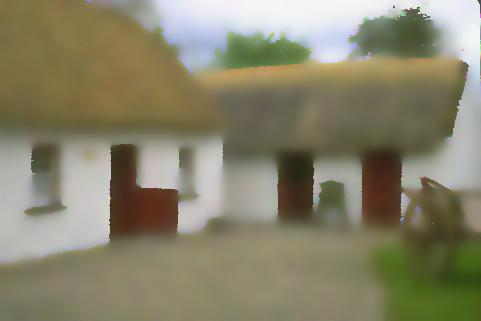
\includegraphics[height=25em]{code/outputs/prob4_1_rep.jpg}
  \caption{Problem 4\_1 repeated result}
  \label{fig:output41rep}
\end{figure*}

\begin{figure*}[!h]
  \centering
    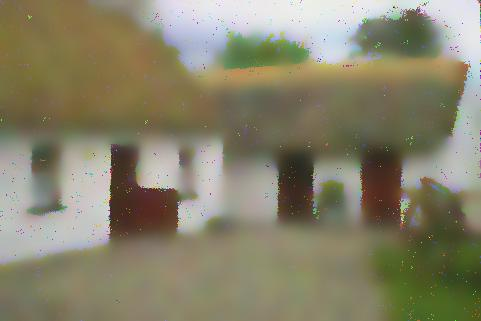
\includegraphics[height=25em]{code/outputs/prob4_2_rep.jpg}
  \caption{Problem 4\_2 repeated result}
  \label{fig:output42rep}
\end{figure*}

\solution{5}
\spart{a} From the slide, we have the discrete 2D Fourier Transform as below:
$$
F[\mu,\nu] = \frac{1}{WH}\sum^{W-1}_{n_x=0}\sum^{H-1}_{n_y=0}X[n_x,n_y] exp(-j2\pi(\frac{\mu n_x}{W}+\frac{\nu n_y}{H}))
$$
we know that $F[\mu,\nu]=F[\mu + W,\nu]=F[\mu,\nu + H]$ because of periodicity, therefore, we typically store $F[\mu,\nu]$ for $\mu \in \{0,...,W-1\}$, $\nu \in \{0,...,H-1\}$. So, within one period, we have $F[-\mu,-\nu]=F[W-\mu,H-\nu]$, which indicates that $F[\mu,\nu]$ is central symmetry, so we can only store half of $F[\mu,\nu]$. The scalars can be stored discuss as follows:
\begin{enumerate}
\item When $W_x$ is even and $H_x$ is even, we can store $\mu \in \{0,...,\frac{W-2}{2}\}$ and $\nu \in \{0,...,H-1\}$, and the other half of the scalars can be recovered by $\mu' = W-\mu$, $\nu'=H-\nu$ for $\mu \in \{0,...,\frac{W-2}{2}\}$ and $\nu \in \{0,...,H-1\}$.
\item When $W_x$ is odd and $H_x$ is even, we can store $\mu \in \{0,...,W-1\}$ and $\nu \in \{0,...,\frac{H-2}{2}\}$, and the other half of the scalars can be recovered by $\mu' = W-\mu$, $\nu'=H-\nu$ for $\mu \in \{0,...,W-1\}$ and $\nu \in \{0,...,\frac{H-2}{2}\}$.
\item When $W_x$ is even and $H_x$ is odd, we can store $\mu \in \{0,...,\frac{W-2}{2}\}$ and $\nu \in \{0,...,H-1\}$, and the other half of the scalars can be recovered by $\mu' = W-\mu$, $\nu'=H-\nu$ for $\mu \in \{0,...,\frac{W-2}{2}\}$ and $\nu \in \{0,...,H-1\}$.
\item When $W_x$ is odd and $H_x$ is odd, we can store $\mu \in \{0,...,\frac{W-1}{2}\}$ and $\nu \in \{0,...,H-1\}$, and the other half of the scalars can be recovered by $\mu' = W-\mu$, $\nu'=H-\nu$ for $\mu \in \{0,...,\frac{W-3}{2}\}$ and $\nu \in \{0,...,H-1\}$.
\end{enumerate}
\spart{b} Figure \ref{fig:output5} is the result of convolution in the Fourier domain.
\begin{figure*}[!h]
  \centering
    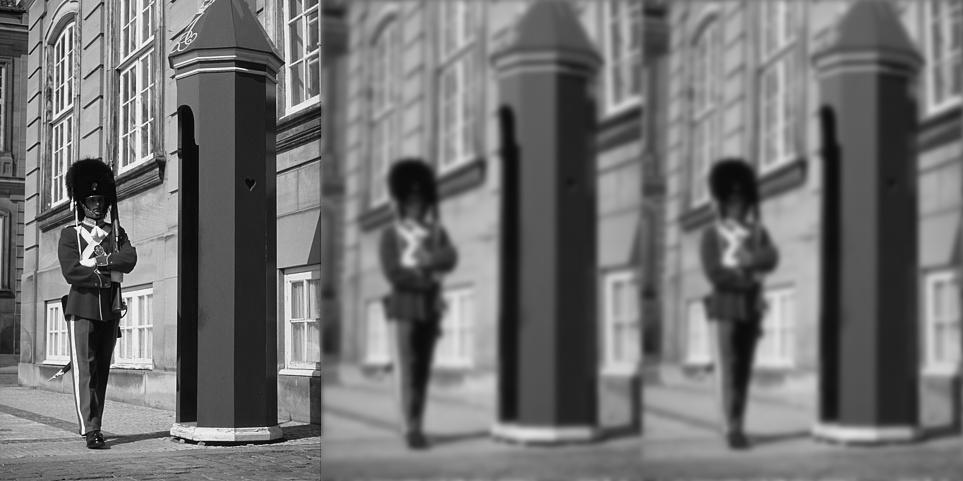
\includegraphics[height=25em]{code/outputs/prob5.jpg}
  \caption{Problem 5 convolution in the Fourier domain}
  \label{fig:output5}
\end{figure*}


\solution{6} 
\spart{a} Figure \ref{fig:output6a} shows the result of Harr wavelet decomposition.
\begin{figure*}[!h]
  \centering
    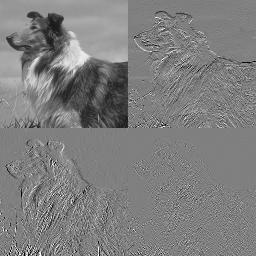
\includegraphics[height=15em]{code/outputs/prob6a_1.jpg}
    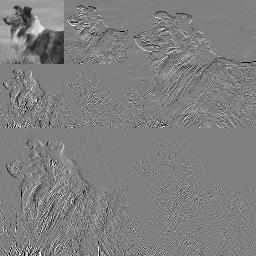
\includegraphics[height=15em]{code/outputs/prob6a_2.jpg}
    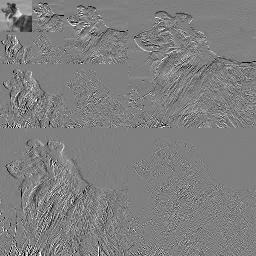
\includegraphics[height=15em]{code/outputs/prob6a_3.jpg}
  \caption{Problem 6a Harr wavelet decomposition}
  \label{fig:output6a}
\end{figure*}

\spart{b} Figure \ref{fig:output6b0} shows the result of reconstruction from Harr wavelet decomposition, and it is fully reconstructed because it is just the same as the original image. Figure \ref{fig:output6b} shows the result of zeroed out the finest levels from 0 to 2.

\begin{figure*}[!h]
  \centering
    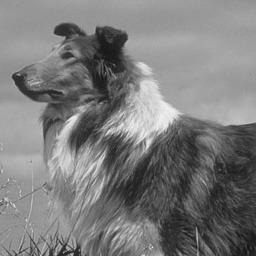
\includegraphics[height=25em]{code/outputs/prob6b.jpg}
  \caption{Problem 6b Reconstruction from Harr wavelet decomposition}
  \label{fig:output6b0}
\end{figure*}

\begin{figure*}[!h]
  \centering
    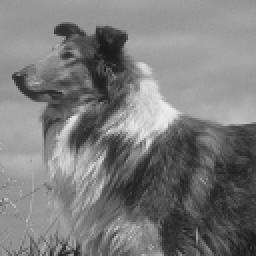
\includegraphics[height=25em]{code/outputs/prob6b_0.jpg}
    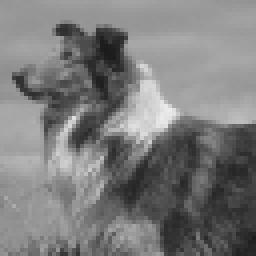
\includegraphics[height=25em]{code/outputs/prob6b_1.jpg}
    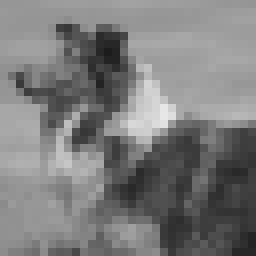
\includegraphics[height=25em]{code/outputs/prob6b_2.jpg}
  \caption{Problem 6b Reconstruction from Harr wavelet decomposition}
  \label{fig:output6b}
\end{figure*}



%%%%%%%%%% Important, you must edit and complete the informational
%%%%%%%%%% section below. If you discussed the problem set with no
%%%%%%%%%% one, edit it to say no discussions or external resources.
\info

This problem set took approximately 42 hours of effort.

I discussed this problem set with:
\begin{itemize}
\item Jiayao Cheng
\item Yukun Li
\end{itemize}

% Note that you might have to escape some special symbols in URLS like \_
I also got hints from the following sources:
\begin{itemize}
\item Wikipedia article on matrix calculus at https://en.wikipedia.org/wiki/Matrix\_calculus
\item Read numpy tutorial from http://cs231n.github.io/python-numpy-tutorial/
\item Read about histogram equalization from https://www.math.uci.edu/icamp/courses/math77c/demos/hist\_eq.pdf
\item Read about grayscale information from https://en.wikipedia.org/wiki/Grayscale
\item Some hints for problem 4 are from TAs and piazza.
\item Read about bilateral filtering from http://www.numerical-tours.com/matlab/denoisingadv\_8\_bilateral/
\end{itemize}

\end{document}
